% LIMIT OF 15 PAGES!

\subsection{Application parallel performance} % typically about 5 pages

\subsubsection{Nek5000/RS and OpenMC: Overview}

We will perform the proposed simulations using NekRS which is a GPU-accelerated
version of Nek5000 (a Gordon Bell and R\&D 100 Prize winner \cite{tufo99a})
that is targeting high performance on forthcoming exascale platforms.  For
performance portability, NekRS is written in C++/OCCA \cite{occa}.  Several key
kernels come from the high-performance OCCA library, libParanumal
\cite{ChalmersKarakusAustinSwirydowiczWarburton2020,streamParanumal2020}, and
have been tailored and expanded to meet the specific requirements of NekRS. 
NekRS retains access to the standard Nek5000 interface, which allows users to
leverage existing user-specific source code such as statistical analysis tools
for turbulence.  NekRS, libParanumal, and OCCA were developed as part of
DOE's ECP in the Center for Efficient Exascale Discretizations (CEED).
NekRS was recognized as a 2023 Gordon Bell Finalist for sustaining $>$28 PFLOPS
as part of a suite of coupled fission/thermal-hydraulics simulations on 72,000
GCDs of Frontier \cite{gb23}.  

A key feature of Nek5000/RS is that optimal communication strategies and
kernels (in the case of NekRS) are chosen at runtime, for each in-situ run
configuration.  These choices are based on trial runs at the start of each
simulation so that the fastest option is chosen according to the actual data
layout.  
For example, for different levels of the $p$-multigrid
(pMG) preconditioner, different communication strategies or different kernels
might be chosen depending on the performance for a given pMG level or processor
count.  {\bf An advantage of this strategy is that there one never experiences
retrograde performance as kernels are updated---if a newer kernel is slower in
some circumstance, the older, faster, one will be selected at run time.}
We remark that highly-tuned fast-diagonalization method (FDM) kernels used in
pMG are reaching 5 TFLOPS on a single GCD of Crusher in FP32, which is used for
preconditioning.   Other kernels are sustaining similar performance, with the
majority of the kernels realizing well above 80\% of the roofline performance.
Including MPI overhead, NekRS is sustaining in excess of 930 GFLOPS FP64 per
A100 on Polaris and 600 GFLOPS on Frontier at modest node counts ($<$1000),
where we count all FP32 flops as 1/2 of an FP64 flop. (See Fig. \ref{fig:flops1}(a).)
For large-system runs,
  the per-node performance on Frontier drops to about 400 GFLOPS/rank because
  of network performance.   We note that the worst of the at-scale network 
  issues, where time-per-step would jump from 0.3 seconds to 10 seconds,
  were largely mitigated by turning off GPU-direct for one of the kernels,
  which reduced network congestion \cite{gb23}
   (Fig. \ref{fig:flops1}(b)--(c)).

%%%%%%%%%%%%%%%%%%%%%%%%%%%%%%%%%%%%%%%%%%%%%%%%%%%%%%%%%%%%%%%%%%%%%%%%%%
\begin{figure} \centering
{\setlength{\unitlength}{1.0in}
   \begin{picture}(6.500,2.000)(0,0.05)
      \put(0.03,0.10){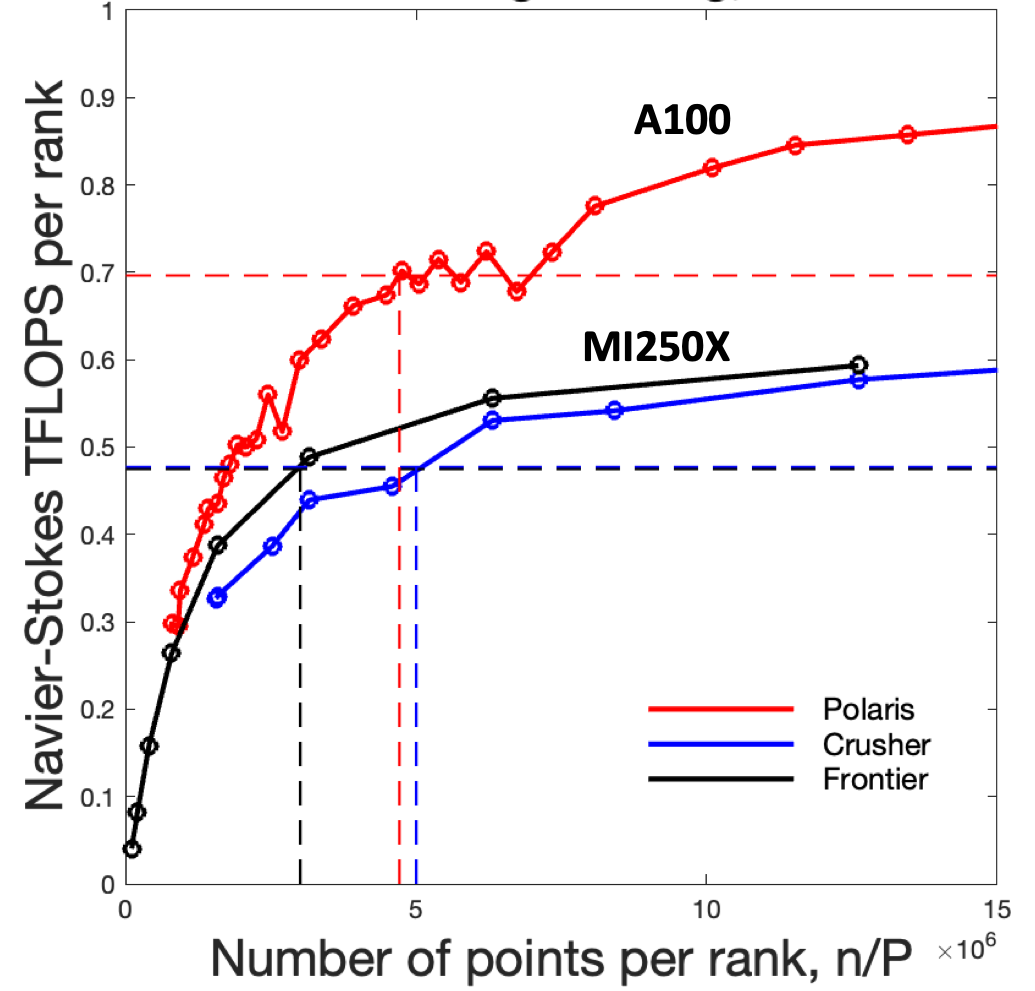
\includegraphics[width=1.68in]{figures/a100_mi250x_flop2.png}}
      \put(1.90,-.05){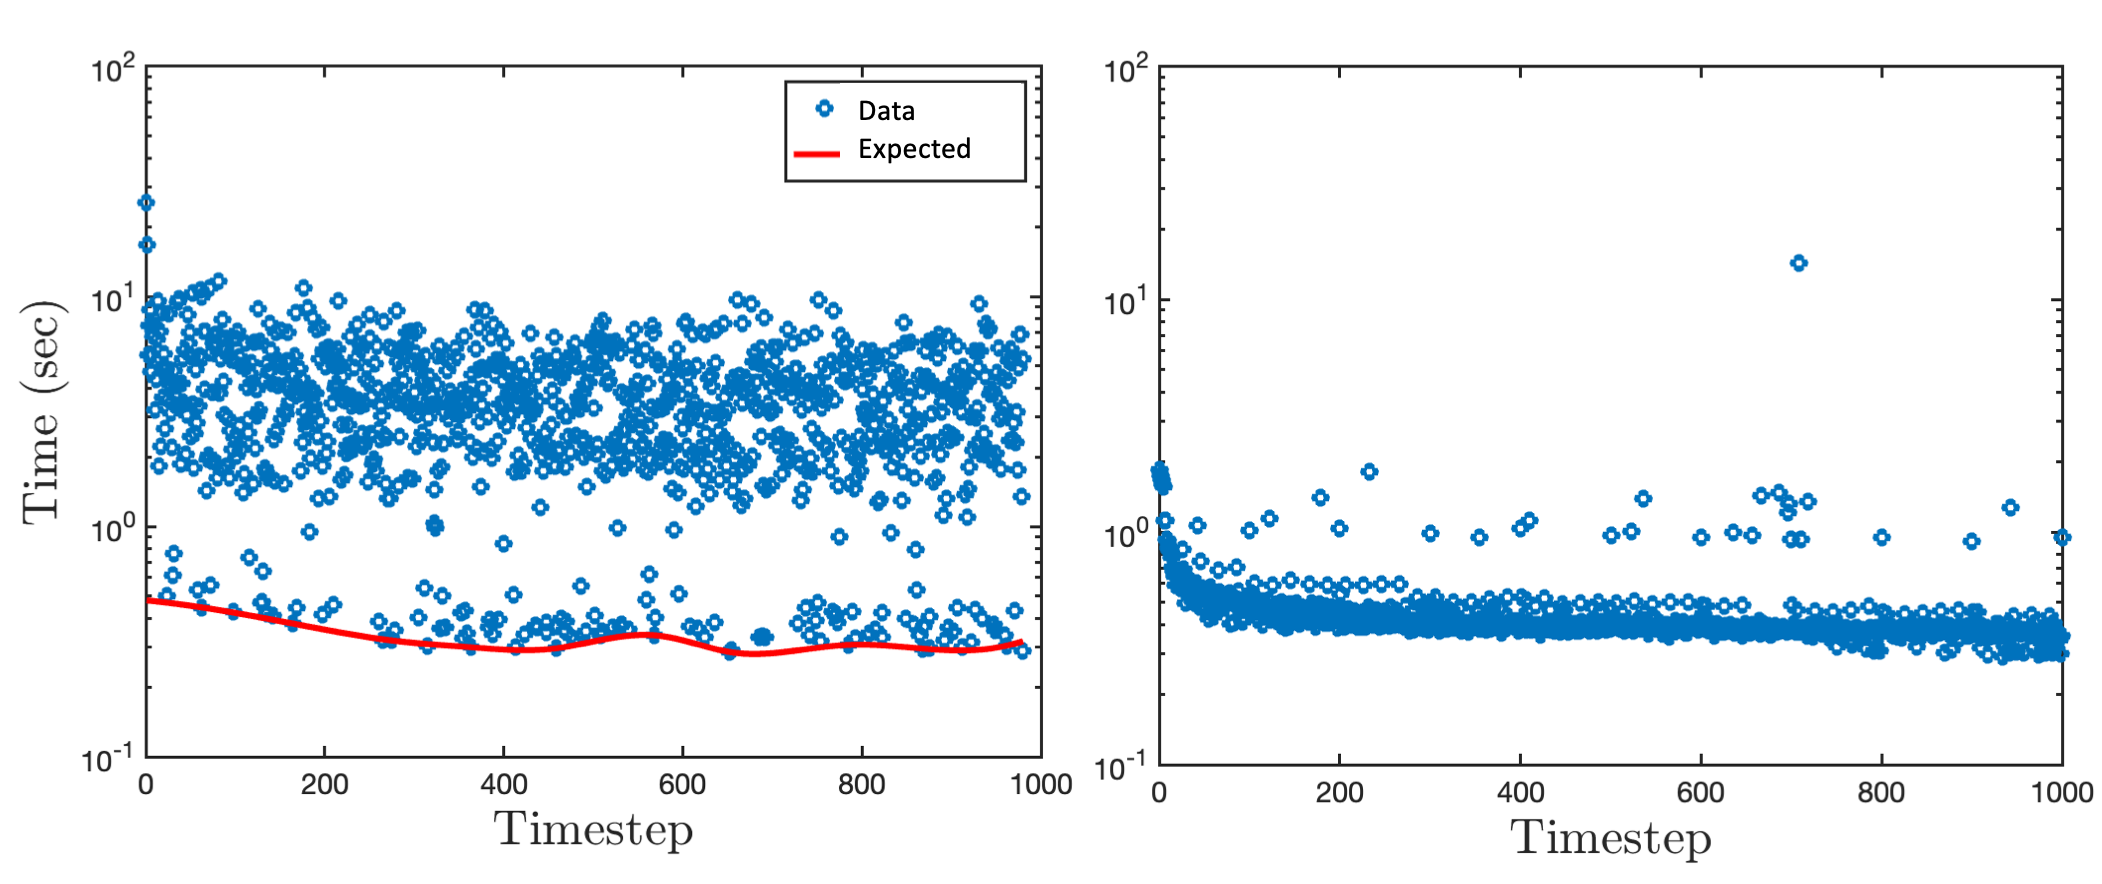
\includegraphics[width=4.50in]{figures/frontier_good_bad.png}}

      \put(0.30,1.55){(a)}
      \put(2.27,1.55){(b)}
      \put(4.46,1.55){(c)}

      \put(0.34,1.8){\small \bf Strong-Scale, $n$=1.6B}
      \put(2.38,1.8){\small \bf Time-per-Step for NekRS on Frontier, $n$=300B, P=72,000 Ranks}
%     \put(2.55,1.8){\small \bf Time-per-Step for NekRS on Frontier, P=72,000 Ranks}


   \end{picture}}
\caption{\label{fig:flops1}\small
(a)
NekRS Navier-Stokes strong-scaling results for a 7th-order,
 ($E,n$)=(4.7M,n=1.6B), spectral
element discretization of a rod-bundle flow using $P=100$--2048 A100 GPUs
and MI250X GCDs. 
  Polaris saturates at 0.93 TFLOPS/rank and realizes $n_{0.8}=5M$, the number of
points per rank where 80\% parallel efficiency is realized.
  Frontier saturates at 0.60 TFLOPS/rank but has $n_{0.8}=3M$. 
At 80\% parallel efficiency, the time-to-solution is lower on Frontier. 
Note that choosing to run Polaris at $\sim$100\% efficiency would result
in a {\em 2.4$\times$ increase in time-to-solution.}
(b)--(c)
Time-per-step for SMR full-core simulations on 9000 nodes of Frontier,
with (b) and without (c) GPU-direct.  
At large node counts, certain communication patterns generate excessive
congestion resulting in the huge jump in time-per-step seen in (b).
Turning off GPU-direct throttles the message flooding and yields 
more than a 10$\times$ performance gain \cite{gb23}.
} 
\end{figure}
%%%%%%%%%%%%%%%%%%%%%%%%%%%%%%%%%%%%%%%%%%%%%%%%%%%%%%%%%%%%%%%%%%%%%%%%%%
%uuuuu


The neutronics portions of simulations are performed using OpenMC, a Monte
Carlo radiation transport code developed as part of the ExaSMR project within
the DOE Exascale Computing Project. 
For performance portability, OpenMC is written in C++ with GPU parallelism via the OpenMP target offloading model ~\cite{Romano2015} 
The LLVM compiler for the OpenMP target offloading model has also been developed as part of the DOE ECP. 
A key benefit of our performance portability strategy is that a single, unified codebase can target GPU architectures developed by all three major vendors (NVIDIA, Intel, and AMD).
This has allowed OpenMC to recently demonstrate exceptional performance on Frontier, Sunspot (the Aurora testbed), and Polaris (a large NVIDIA GPU-based system at Argonne).

\subsubsection{Nek5000/RS: Perfomance}

\noindent{\bf State-of-the-Art.}
Nek5000/RS is based on the spectral element method (SEM) \cite{pat84}, in which
functions are represented as $N$th-order polynomials on each of $E$ elements,
for a total mesh resolution of $n=EN^3$.  
The SEM offers many advantages for this class of problems.  It accommodates
body-fitted coordinates through isoparametric mappings domain from the
reference element, $\Oh:=[-1,1]^3$ to the individual (curvilinear-brick)
elements $\Omega^e$.  On $\Oh$, solutions are represented in terms of
$N$th-order tensor-product polynomials,
\begin{eqnarray} \label{eq:field1}
\left. {\bf u}({\bf x}) \right|^{}_{\Omega^e} = \sum_{i=0}^N
\sum_{j=0}^N \sum_{k=0}^N {\bf u}_{ijk}^{e}\,h_i(r)\,h_j(s)\,h_k(t),
\end{eqnarray}
where the $h_i$s are stable nodal interpolants based on the
Gauss-Lobatto-Legendre (GLL) quadrature points $(\xi_i,\xi_j,\xi_j)\in \Oh$
and ${\bf x}={\bf x}^e(r,s,t)$ on $\Omega^e$.
This form allows all operator evaluations to be expressed as {\em fast tensor
contractions}, which can be implemented as BLAS3 operations\footnote{For
example, with $\Dh_{il} := \dd{h_l}{r} |^{}_{\xi_i}$,
the first derivative takes the form $u_{r,ijk}=\sum_l \Dh_{il} u_{ljk}$,
which is readily implemented as an $N_p \times N_p$ matrix times
an $N_p \times N_p^2$ matrix, with $N_p=N+1$.}
in only $O(N^4)$ work and $O(N^3)$ memory references \cite{dfm02,sao80}.
This low complexity is in sharp
contrast to the $O(N^6)$ work and storage complexity of the
traditional $p$-type FEM.  Moreover, hexahedral (hex) element function
evaluation is about six times faster per degree-of-freedom (dof) than
tensor-based tetrahedral (tet) operator evaluation \cite{moxey20}.
By diagonalizing one direction at a time, the SEM structure admits
fast block solvers for local Poisson problems in undeformed and (approximately)
in deformed elements, which serve as local smoothers for $p$-multigrid (pMG)
\cite{lottes05}.

$C^0$ continuity implies that the SEM is {\em communication minimal:}
data exchanges have unit-depth stencils, independent of $N$.
Finally, local $i$-$j$-$k$ indexing avoids much of the indirect addressing
associated with fully unstructured approaches, such that high-order SEM
implementations can
realize significantly higher throughput (millions of dofs per second, MDOFS)
than their low-order counterparts \cite{ceed_bp_paper_2020}.

\input tex/figscale_crop




\paragraph{Aurora performance.} 
From the logfile timing data, we plot strong-scaling performance in Fig.
\ref{fig:scale} for a flow through a single $17 \times 17$ rod bundle of a
fission reactor for $E=4709$K elements of order $N=7$ ($n$=1.6B gridpoints).
Shown in the top row are measured values of the time-per-step for three
platforms: OLCF's Frontier, which features AMD MI250X GPUs, each having two MPI
ranks (one per GCD); ALCF's NVIDIA A100-based Polaris (one rank per A100); and
ALCF's Aurora, which has Intel PVC GPUs, each running two MPI ranks (one per
tile).  We plot the performance as a function of $P$, the number of MPI ranks,
in the upper left, and as a function of $n/P$ on the upper right.  Because it
factors out problem size, the number of points per rank is somewhat more
universal than the number of ranks as an independent variable
\cite{ceed_bp_paper_2020}.  The plots show that Polaris is about $2\times$
faster than Aurora, per rank and about $1.5 \times$ faster than Frontier.  We
expect that the Aurora numbers will improve as network issues are sorted out.
%
%The center row shows the parallel efficiency. We see that, for this case,
%
Inspection of the data reveals that
Frontier realizes $\approx 80$\% efficiency at $n_{0.8}=n/P=4$M points per
rank, whereas Polaris has $n_{0.8} = 5$M, and Aurora has $n_{0.8}=7$M.  
Larger values of $n_{0.8}$ imply that one has to use fewer processors, and thus
run slower, to maintain 80\% efficiency. (Small $n_{0.8}$ is better.)  In all
likelihood, Aurora's numbers will improve once this early system is debugged.


The last row of Fig. \ref{fig:scale} breaks out the costs of some of the
leading performance bottlenecks.  On the lower left, we plot the time-per-step
for the nonlinear advection evaluation, {\tt makef}.  We see that Aurora spends
roughly twice the amount of time in this kernel than either Frontier or
Polaris.  This kernel shows perfect linear scaling because it is compute
intensive and almost devoid of communication.  We speculate that the relatively
poor performance of Aurora stems from cache effects on the PVC.  Because
advection is dealiased with the 3/2's rule, the working data set per element is
$12^3$, rather than $8^3$, which is the size for the majority of the other
elemental operations.  Experiments in which we reduce the order of dealising
from 12 to 9 for this case led to a 1.5$\times$ reduction in advection time,
but this is not as dramatic an improvement as one might expect when cache
spilling is alleviated.  We note that the majority of the Aurora kernel
performance is on par with Frontier.

\subsubsection{MHD performance study}

\input tex/mhd_performance

\subsubsection{OpenMC: Performance}

The stochastic, direct simulation approach used in OpenMC is extremely computationally expensive in that a large quantity of particles must be simulated to reduce stochastic uncertainties to acceptable levels. 
The algorithm's stochastic nature requires special attention to map efficiently to modern computer architectures due to ample use of conditional branching logic and highly random memory access patterns inherent in sampling large tables of probabilistic distribution data. %For these reasons, fields that involve neutral particle transport simulation often use faster, but less accurate and less general deterministic methods. The assumptions and discretizations used in deterministic methods often result in the need for highly complex (and problem-specific) correction factors, meaning that deterministic applications typically only work within a very narrow problem space. 
%Thus, in many fields of particle transport, engineers are typically limited in their ability to evaluate new or novel designs.
%To this end, the recent decade has seen a significant increase in interest in using the more general and more accurate Monte Carlo method for routine design and engineering simulation work across a variety of fields. Two fields of interest is neutron transport simulations of full nuclear reactor cores (particularly in a multphysics context), as well as neutron transport in multiphysics simulations of complex fusion devices. 
%The extremely high computational cost of using the Monte Carlo method for such simulations makes these problems ideal use cases for exascale class supercomputers. 
OpenMC, developed as part of the ECP ExaSMR project, performs Monte Carlo particle transport simulations efficiently on exascale systems from all major GPU vendors~\cite{Tramm2022}. 

%\begin{wraptable}{r}{8cm}
%\vspace{-1em}
%	\centering
%	\small
%	\caption{Key parameters for benchmark problem used to assess OpenMC performance}
%	\label{tab:smr}
%	\begin{tabular}{@{}ll@{}}
%		\toprule
%		Parameter                              & Value   \\ \midrule
%		Number of unique materials             & 195,368  \\
%		%Number of unique fuel materials        & 195,360 \\
%		Number of depletion tally regions      & 195,360 \\
%		Number of nuclides in each fuel region & 244     \\
%		%Number of nuclides in simulation       & 281     \\ 
%		\bottomrule
%	\end{tabular}
%\end{wraptable}

Here, we present results for OpenMC run at scale on the Crusher, Sunspot, and Polaris systems to demonstrate OpenMC's readiness on these systems, plus the readiness of the OpenMP target offloading compiler toolchains that used to support these runs. All performance numbers in this section are assessed using a large, representative benchmark problem of a full-size, realistic SMR geometry using 195,000 materials and 195,000 tallies \cite{ecp-se-08-43}. The high expense of 
looking up fuel cross sections for hundreds of nuclides is representative of the challenge problems identified in this proposal.
To demonstrate the performance portability at scale we utilize the leadership class supercomputing systems Polaris, Crusher, and Sunspot.

\vspace{-.15in}
\paragraph{Single GPU and Single Node Performance}

%We evaluate the GPU- and node-level performance of OpenMC on the Sunspot, Crusher, and Polaris systems. 
We measured performance on a single GPU NUMA region (i.e., one PVC tile or one MI250X GCD), a single GPU (i.e., one A100, two PVC tiles, or two MI250X GCDs), a single node using all available GPUs, and a single node using only the host multicore CPUs. 
As shown in \autoref{fig:node_compare}, OpenMC runs highly efficiently on A100, MI250X, and PVC GPUs. We found that a single PVC was over twice as fast as a single A100 GPU. A single MI250X was slightly faster than the A100. 

%%%UUU
\begin{figure*}[h]
	\centering
	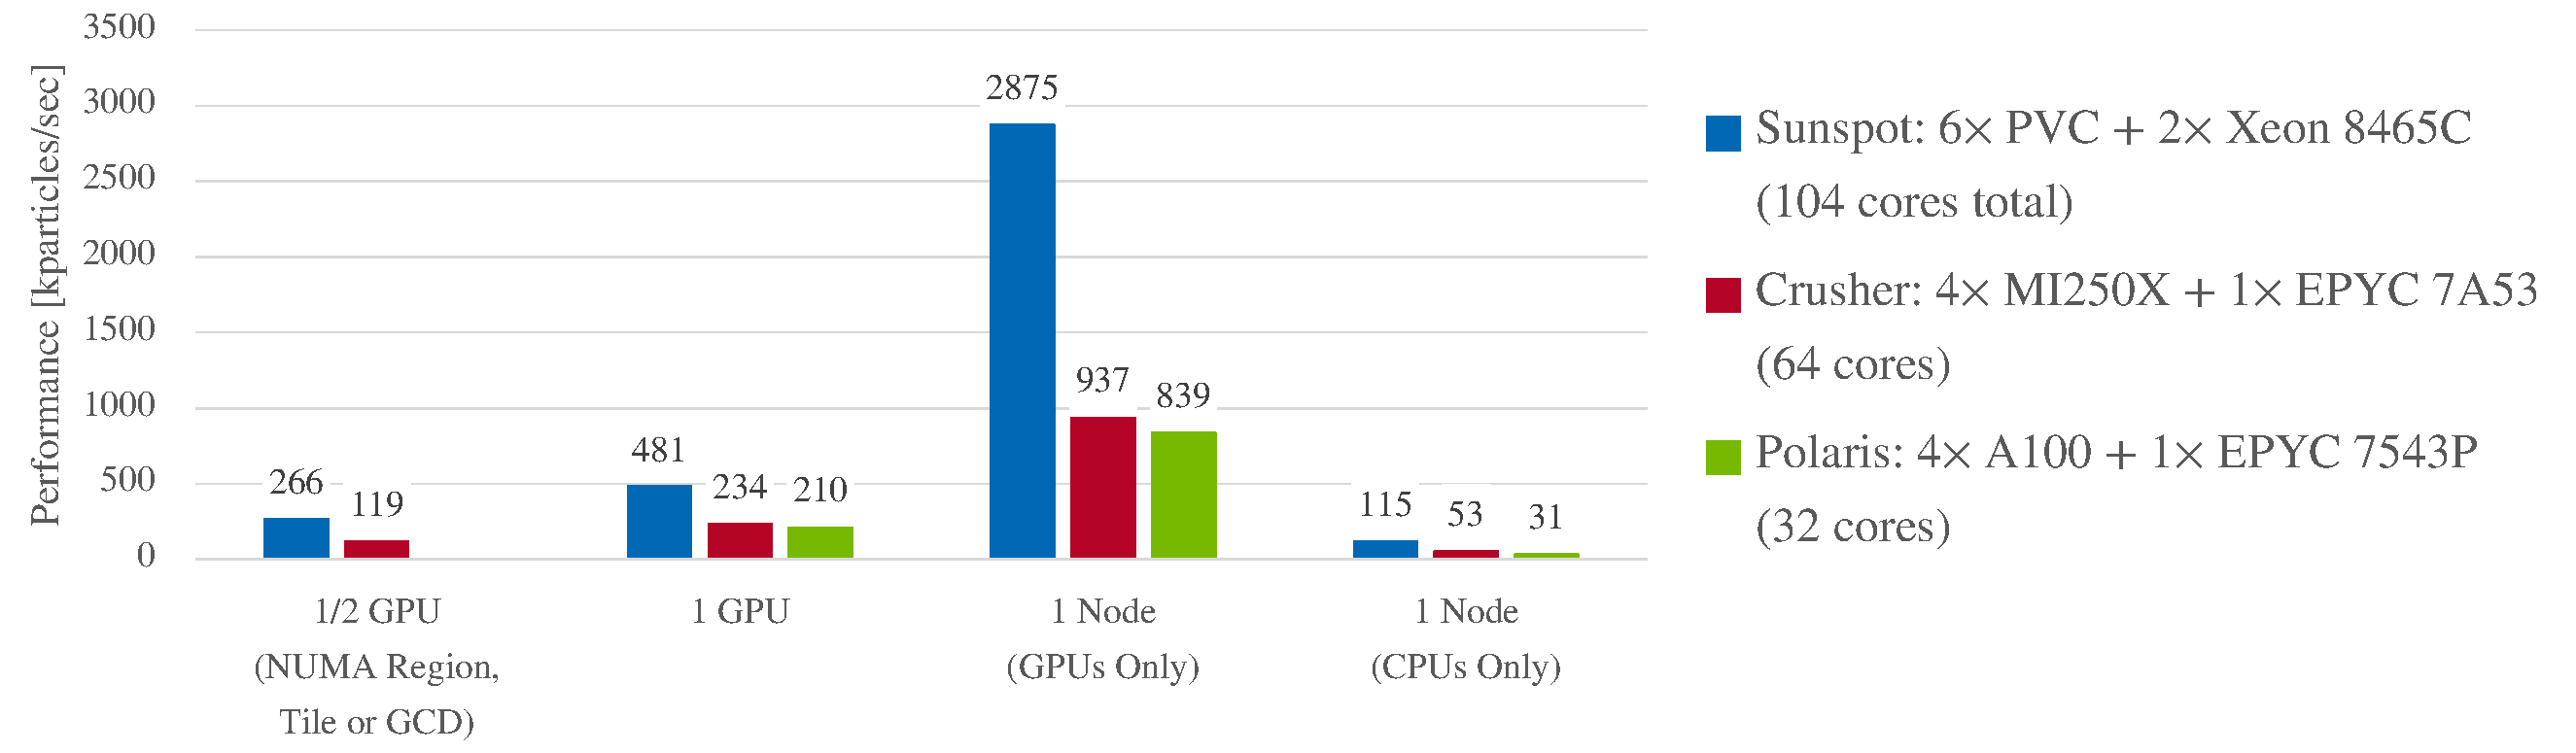
\includegraphics[width=0.9\linewidth]{figs/openmc_node_compare_slim.pdf}
	\caption{\small Performance (particles/second) comparison of OpenMC on various architectures.}
	\label{fig:node_compare}
\end{figure*}

All GPUs on each node afforded a 18--27$\times$ speedup as compared to running
OpenMC on the multicore host CPUs alone. Use of a single GPU on each node
resulted in a speedup of 3.5--6.7$\times$ compared to using all CPUs on the
host node. These results show that OpenMC is making good use of the system's
GPUs.  Furthermore, the OpenMP offloading port of OpenMC was done in a manner
that allowed for reproducible solutions that were identical with those
generated by OpenMC before the porting effort began \cite{Tramm2022}.

%However, absent a theoretical performance model, one natural question that arises with such CPU vs. GPU comparisons is whether or not the CPU version of the code is reasonably well optimized. Later in this paper, in \autoref{sec:code_compare}, we will show that OpenMC performs well on CPU as compared to other state-of-the-art MC 
applications---indicating that the demonstrated GPU speedups over CPU are not
caused by a deficient CPU implementation.


\vspace{-.15in}
\paragraph{Many Node Performance}
The MPI communication patterns used by OpenMC typically result in very low
communication costs on CPU-based architectures. However, given the massive
improvements in node-level particle tracking rates that GPUs offer, it is
important to evaluate OpenMC at scale to determine if communication costs have
become relatively more expensive.  We tested OpenMC's weak scaling performance
out to 96 GPUs, which corresponds to 24 nodes of Polaris or Crusher and 16
nodes of Sunspot. \autoref{fig:weak_scaling}(a) indicates that the total
particle tracking rate appears to increase in a nearly ideal fashion out to 96
GPUs for all three systems. %The x-axis of the scaling plot is given in terms
of GPUs instead of nodes due to the Sunspot node architecture featuring 6 GPUs,
while the Crusher and Polaris node architectures only feature 4 GPUs.  In
\autoref{fig:weak_scaling}(b), the weak scaling data is plotted in terms of
weak scaling efficiency (baselined off of single GPU performance) instead of
absolute tracking rate. The three systems are shown to offer very high levels
of weak scaling efficiency at the 96 GPU level, with values of around 98--99\%,
thereby proving that communication costs for OpenMC remain low even on powerful
multi-GPU node architectures.

%%%UUU
\begin{figure}[!htb] \centering
\begin{subfigure}{0.45\textwidth}
  \centering
 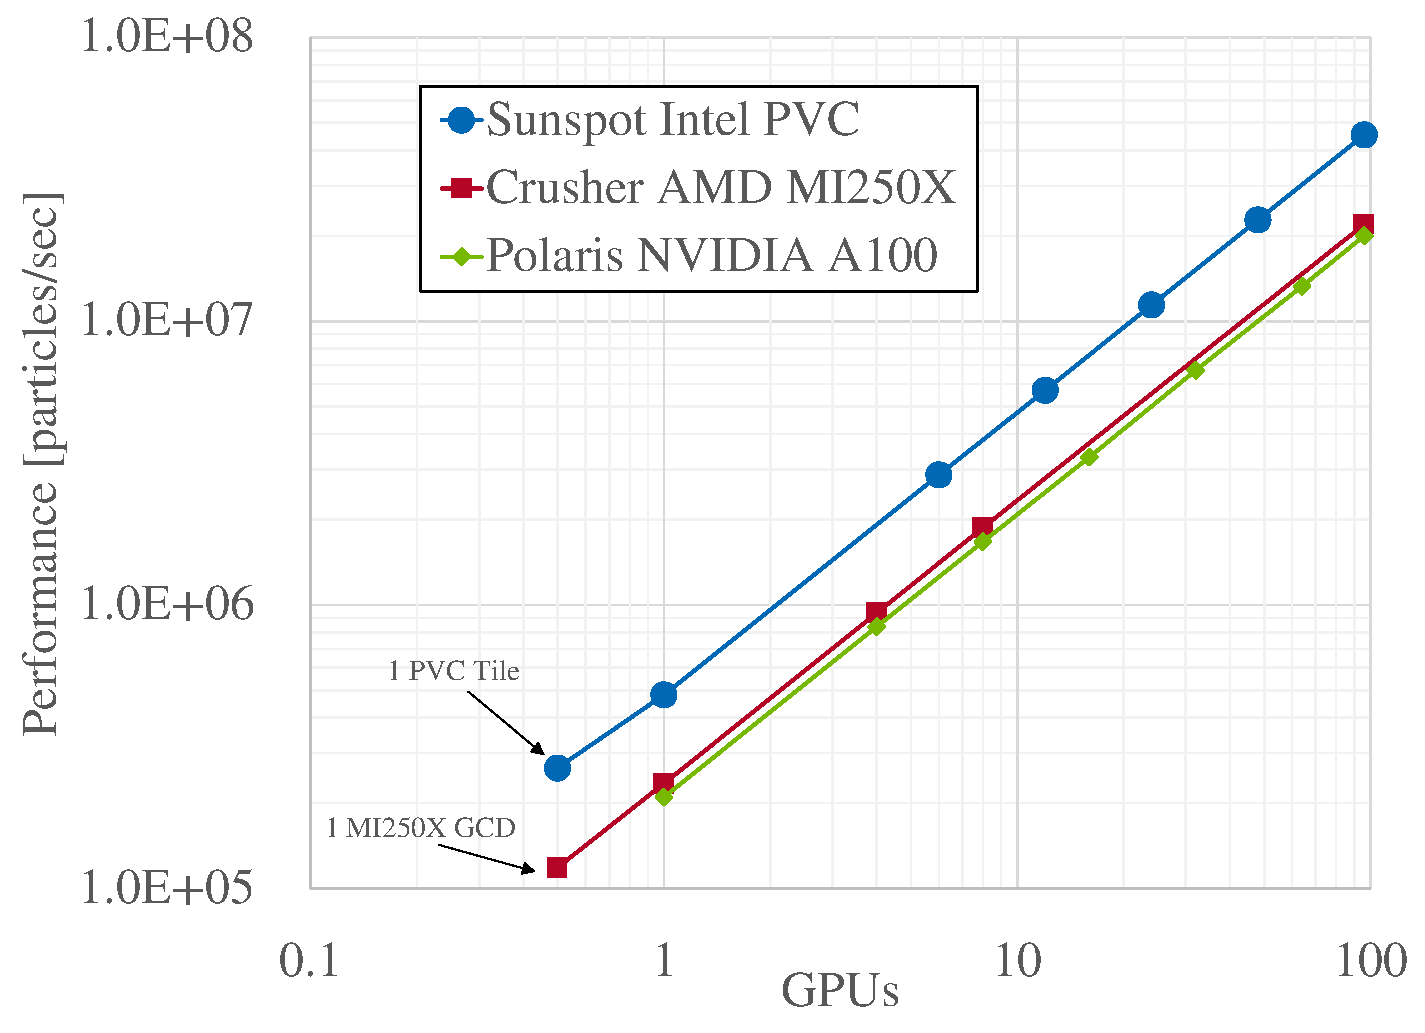
\includegraphics[width=\linewidth]{figs/openmc_weak_scaling_absolute.pdf}
  \caption{Particles/sec}
\end{subfigure}
\begin{subfigure}{0.45\textwidth}
  \centering
 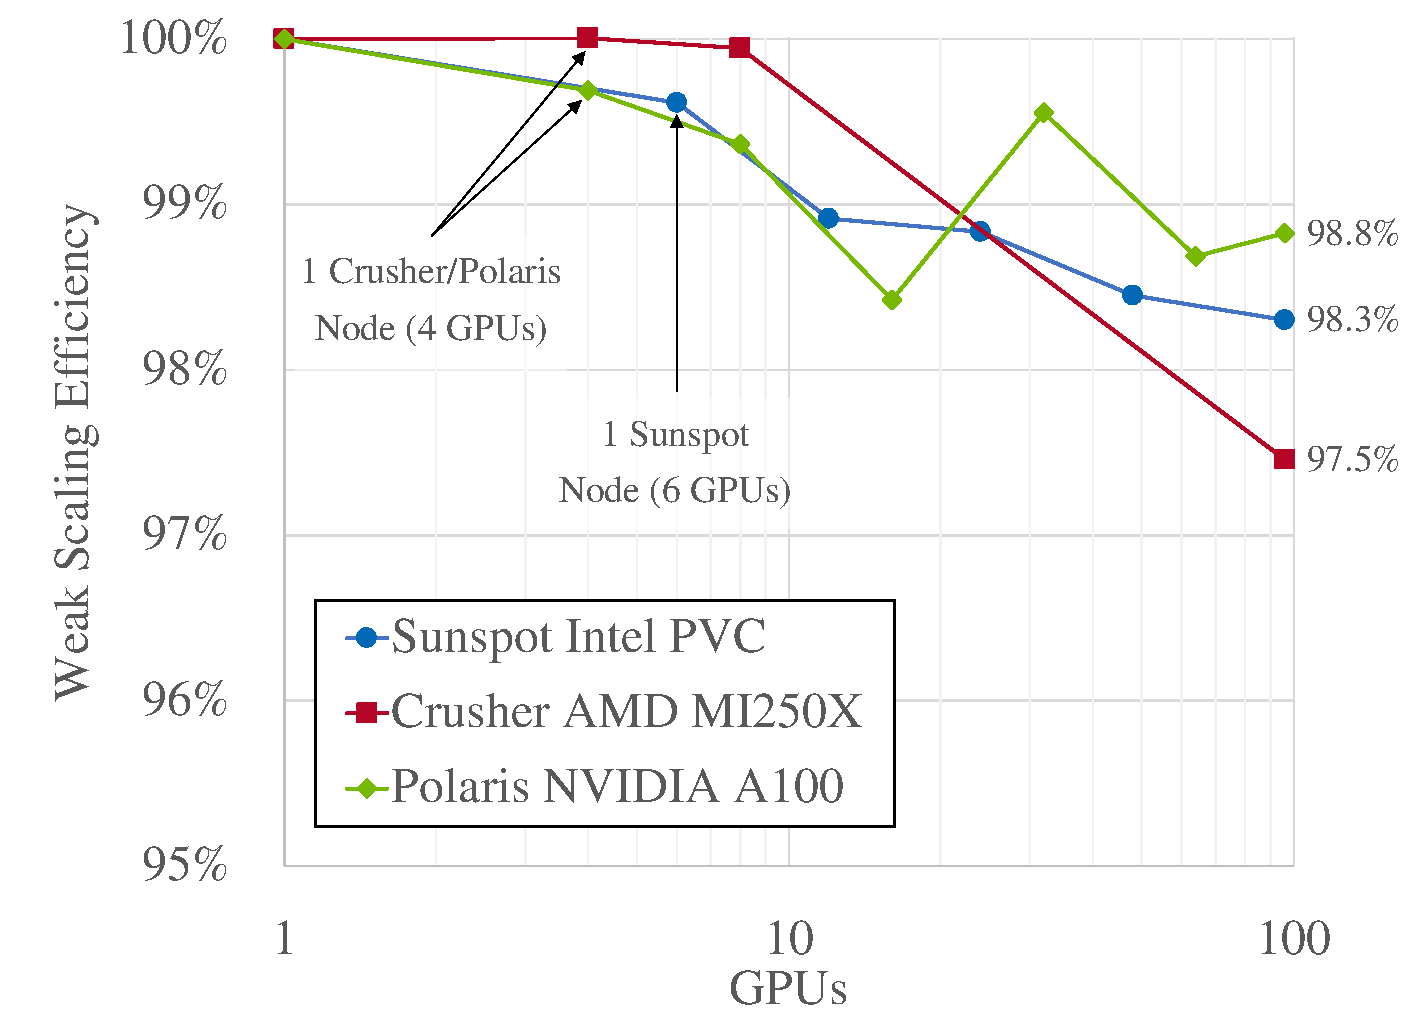
\includegraphics[width=\linewidth]{figs/openmc_weak_scaling_efficiency.pdf}
  \caption{Weak scaling efficiency}
\end{subfigure}
\caption{\small Weak scaling performance (particles/sec) of 
         OpenMC on various architectures.  } 
\label{fig:weak_scaling}
\end{figure}

%\paragraph{Performance Summary}

%Another key finding was that OpenMC was in fact capable of running efficiently
%on GPUs from Intel, NVIDIA, and AMD using the OpenMP target offloading model.
%For instance, 
In summary, using all GPU node resources on the Sunspot, Crusher, and Polaris
systems yielded massive speedups as compared to running OpenMC on the CPU
resources of the nodes. At the node level, Sunspot's six Intel PVC GPUs were in
aggregate 25$\times$ faster than its dual-socket, 104 core Sapphire Rapids Xeon
host CPUs. Crusher's four MI250X GPUs were in aggregate about 18$\times$ faster
than its 64 core AMD EPYC host CPU. Polaris' four A100 GPUs were in aggregate
27$\times$ faster than its 32 core AMD EPYC host CPU. That is, OpenMP target
offloading allowed OpenMC to make excellent use of each system's GPUs---an
impressive feat given how high-level and expressive the OpenMP programming
model is.  We also note that we have more recently been able to replicate the
performance observed on Crusher on Frontier itself. Therefore, our high
readiness level on Crusher is confirmed to translate directly to Frontier.

%\vspace{-.15in}
%\paragraph{Project Workflow and I/O}
%Input files for OpenMC are composed of XML model definition files and cross
%section data HDF5 files. The XML inpus are typically on the order of kilobytes
%to megabytes, and the cross section data files are on the order of tens of
%gigabytes. As they are each read only once at program initialization, file I/O
%for reading this data is not expected to be intensive at all. For the
%simulations discussed in this proposal, output tally data (in the form of HDF5
%statepoint files emitted from OpenMC once at the conclusion of each
%simulation) will be at most about 100 GB each, although we expect sizes will
%more likely to be on the order of just hundreds of megabytes given the
%specifics of the tally phase space that these problems will require. The
%outputting of data files is not expected to be an expensive or intensive I/O
%operation, as it is just performed once at the conclusion of the simulation.
%OpenMC does support checkpointing and restarting via HDF5 statepoint files,
%but we do not expect to use these features as part of our workflow on this
%project. Data analysis and visualization on end-of-simulation statepoint HDF5
%statepoint files will be performed using OpenMC's python data visualization
%interface, and is not expected to require intensive computing, I/O, or disk
%storage resources.
%


